\documentclass[10pt,a4paper]{article}
\usepackage[spanish,es-noshorthands]{babel}
\usepackage[utf8]{inputenc}
\usepackage[T1]{fontenc}
\usepackage{geometry}
\usepackage{listings}
\usepackage{graphicx}
\usepackage{caption}
\usepackage{xurl}
\usepackage{hyperref}
\geometry{margin=1.35cm}
\setlength{\parskip}{0.22em}
\setlength{\parindent}{0pt}
\hypersetup{colorlinks=true,urlcolor=blue,linkcolor=black}
\captionsetup{font=scriptsize,skip=2pt}
\lstset{basicstyle=\ttfamily\scriptsize,breaklines=true,frame=single,columns=fullflexible,keepspaces=true,aboveskip=2pt,belowskip=2pt}

\title{\vspace{-1.4em}Mantenimiento de Gilded Rose\\{\large Actividad 2, Unidad 2}}
\author{Manuel Lozano}
\date{17 de octubre de 2026}

\begin{document}
\maketitle
\vspace{-2.4em}

\section{Introducción y selección del código}
El caso de clase es ConstruYA, una cadena de ferreterías cuyo inventario acumula deuda técnica: un cambio, como integrar una pasarela de pagos, tarda más y puede introducir fallas. El componente intervenido es el inventario de la tienda Gilded Rose, kata de Emily Bache en Python (\url{https://github.com/emilybache/GildedRose-Refactoring-Kata}). Cumple el mismo papel: una regla de negocio nueva es una solicitud de cambio. La licencia original se conserva. La clase \texttt{Item} y la propiedad \texttt{items} no se modifican.

El código que no es prueba suma 80 líneas: 46 en \texttt{gilded\_rose.py} y 34 en \texttt{texttest\_fixture.py}. El conteo está en la evidencia. No llega al mínimo de 150 que pide el procedimiento. No se añadió código de relleno. La figura~\ref{fig:entorno} muestra las versiones del entorno, renderizadas desde esa evidencia.

\begin{figure}[!htbp]
\centering
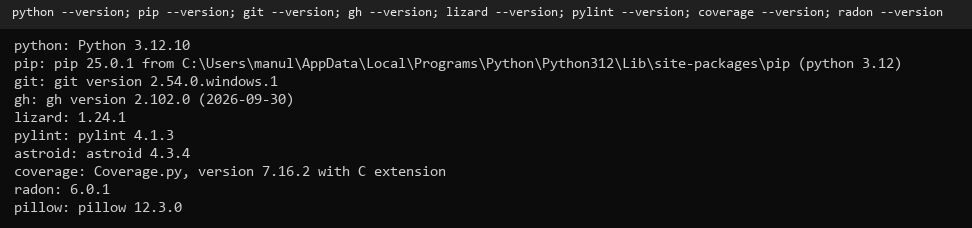
\includegraphics[width=\textwidth]{imagenes/01_entorno.png}
\caption{Salida de los comandos de versión (Python, pip, git, gh, lizard, pylint, coverage, radon y pillow), tomada de \texttt{evidencia/entorno.txt}.}
\label{fig:entorno}
\end{figure}

\section{Diagnóstico}
pylint~4.1.3, sobre \texttt{gilded\_rose.py} y \texttt{texttest\_fixture.py}, calificó el original con 6.48/10 (figura~\ref{fig:pylint-antes}). No marca método largo, números mágicos ni clones. lizard~1.24.1 con \texttt{-C 10 -L 50} sí marca \texttt{update\_quality}: NLOC 29, CCN 19, longitud 29 (figura~\ref{fig:lizard-antes}). La longitud no supera 50; el aviso es por la complejidad.

\begin{figure}[!htbp]
\centering
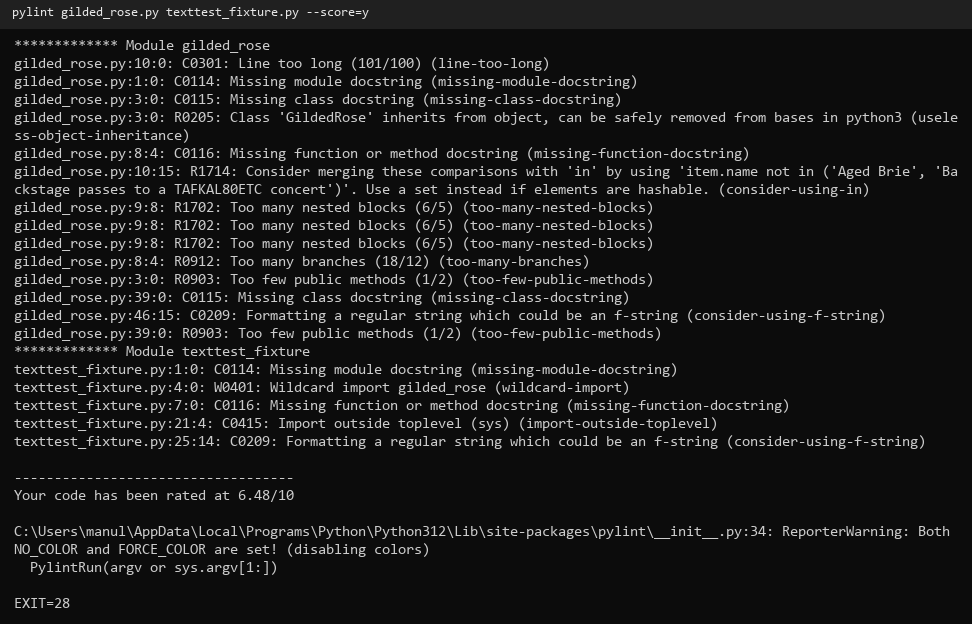
\includegraphics[width=\textwidth]{imagenes/02_pylint_antes.png}
\caption{Salida de \texttt{pylint gilded\_rose.py texttest\_fixture.py --score=y} antes de refactorizar.}
\label{fig:pylint-antes}
\end{figure}

\begin{figure}[!htbp]
\centering
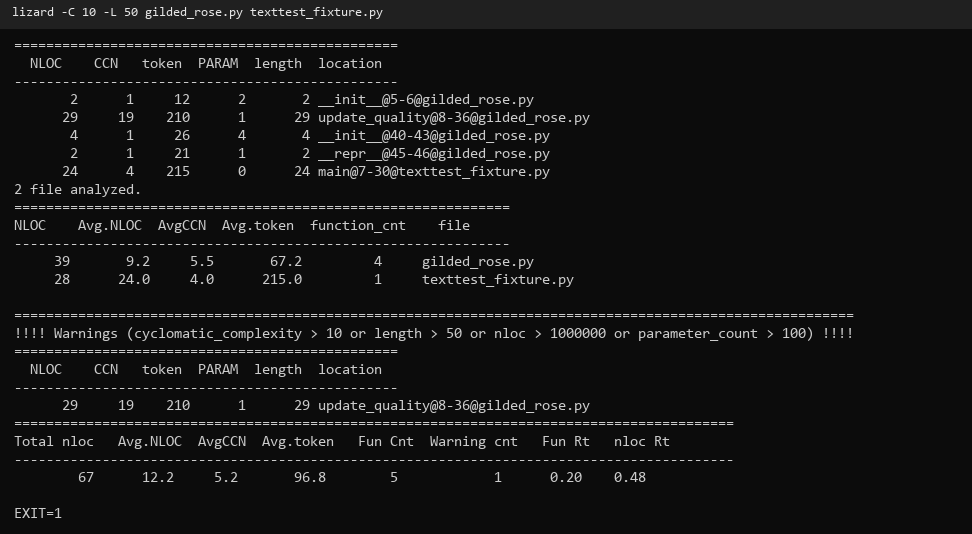
\includegraphics[width=\textwidth]{imagenes/03_lizard_antes.png}
\caption{Salida de \texttt{lizard -C 10 -L 50 gilded\_rose.py texttest\_fixture.py}.}
\label{fig:lizard-antes}
\end{figure}

\begin{center}
\scriptsize
\begin{tabular}{|p{2.6cm}|p{2.5cm}|p{4.4cm}|p{4.6cm}|}
\hline
Smell & Ubicación & Evidencia & Técnica \\
\hline
Método con demasiadas ramas & \texttt{update\_quality}, 8--36 & lizard CCN 19. pylint R0912: 18/12 & Extraer método y estrategia \\
\hline
Condicionales anidados & líneas 9--36 & pylint R1702: 6/5, tres veces & Guardas y retorno temprano \\
\hline
Números mágicos & 0, 50, 11 y 6 & pylint no los marca; inspección & Constantes con nombre \\
\hline
Cadenas repetidas & Brie, Sulfuras, Backstage & pylint R1714 solo en la línea 10 & Constantes con nombre \\
\hline
Duplicación al subir o bajar calidad & líneas 13, 16, 20, 23, 31 y 36 & sin detector de clones; inspección & Métodos con límite \\
\hline
Tipo de producto como cadena & comparaciones de \texttt{name} & ninguna herramienta lo nombra & Despacho por estrategia \\
\hline
\end{tabular}
\end{center}

\section{Refactorización}
Cinco técnicas, un commit cada una, en \texttt{refactor/gilded-rose}. Tras cada una, las 13 pruebas siguieron en verde. El golden master no se regeneró.

Antes, la regla y el límite vivían en el mismo bloque:

\begin{minipage}{\textwidth}
\begin{lstlisting}
if item.quality > 0:
    if item.name != "Sulfuras, Hand of Ragnaros":
        item.quality = item.quality - 1
\end{lstlisting}
\end{minipage}

Después, el límite está en una función y el tipo se elige en un diccionario (\texttt{actualizadores.py}):

\begin{minipage}{\textwidth}
\begin{lstlisting}
def bajar_calidad(item):
    if item.quality > MIN_QUALITY:
        item.quality = item.quality - 1

DESPACHO = {
    AGED_BRIE: actualizar_brie,
    BACKSTAGE_PASSES: actualizar_backstage,
    SULFURAS: actualizar_sulfuras,
}
\end{lstlisting}
\end{minipage}

\texttt{update\_quality} quedó en 3 líneas de código, CCN 2 y longitud 3 (figura~\ref{fig:lizard-despues}). Las otras técnicas fueron constantes con nombre, métodos por tipo de ítem y cláusulas de guarda. Los fragmentos están en \texttt{evidencia/refactor\_1\_antes.txt} a \texttt{refactor\_5\_despues.txt}.

\section{Herramientas de análisis estático y dinámico}
La estática es pylint, complementada con lizard. La dinámica es coverage.py con \texttt{--branch}. No se usa la cobertura como prueba de que el diseño mejoró: con 5833 combinaciones y 40 días, el original ya cubría todas las ramas ejecutables.

\begin{center}
\scriptsize
\begin{tabular}{|p{4.3cm}|p{5.4cm}|p{5.4cm}|}
\hline
Métrica & Antes & Después \\
\hline
\texttt{update\_quality} & NLOC 29, CCN 19, longitud 29 & NLOC 3, CCN 2, longitud 3 \\
\hline
CCN media (lizard) & 5,2; una función sobre el umbral & 1,9; ninguna sobre el umbral \\
\hline
pylint & 6,48/10; 19 avisos & 6,94/10; 22 avisos \\
\hline
Cobertura & 36 sentencias, 1 sin cubrir, 34 ramas, 99\,\% & 54 sentencias, 1 sin cubrir, 16 ramas, 99\,\% \\
\hline
Pruebas & 13, todas OK & 13, todas OK \\
\hline
\end{tabular}
\end{center}

Los avisos de pylint suben de 19 a 22 porque las funciones nuevas no tienen docstring y el import estrella marca \texttt{actualizar\_item}. Desaparecen R1702 y R0912. Las ramas bajan de 34 a 16 porque se eliminó código duplicado, no porque las pruebas dejen de recorrer reglas. La línea sin cubrir sigue siendo \texttt{\_\_repr\_\_}. Figuras~\ref{fig:cobertura-antes} y~\ref{fig:cobertura-despues}.

\begin{figure}[!htbp]
\centering
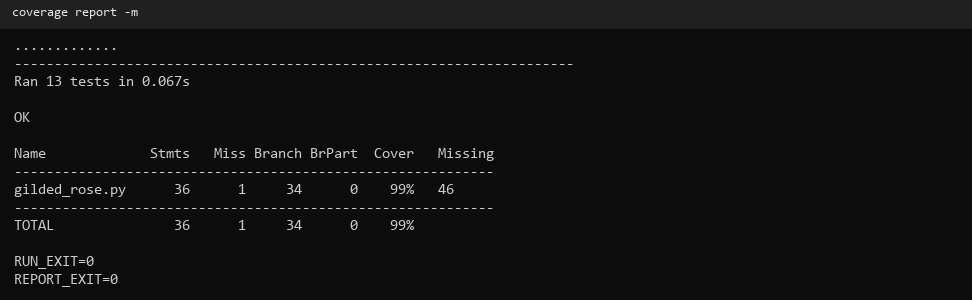
\includegraphics[width=\textwidth]{imagenes/05_cobertura_antes.png}
\caption{Salida de \texttt{coverage report -m} antes de refactorizar.}
\label{fig:cobertura-antes}
\end{figure}

\begin{figure}[!htbp]
\centering
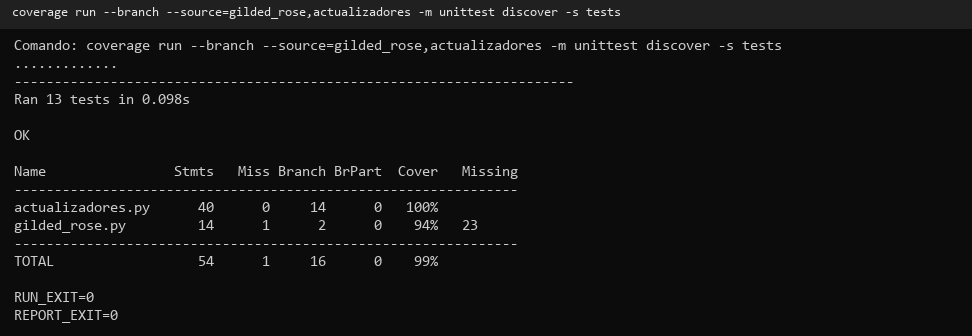
\includegraphics[width=\textwidth]{imagenes/09_cobertura_despues.png}
\caption{Salida de \texttt{coverage run --branch --source=gilded\_rose,actualizadores} y del reporte posterior.}
\label{fig:cobertura-despues}
\end{figure}

\begin{figure}[!htbp]
\centering
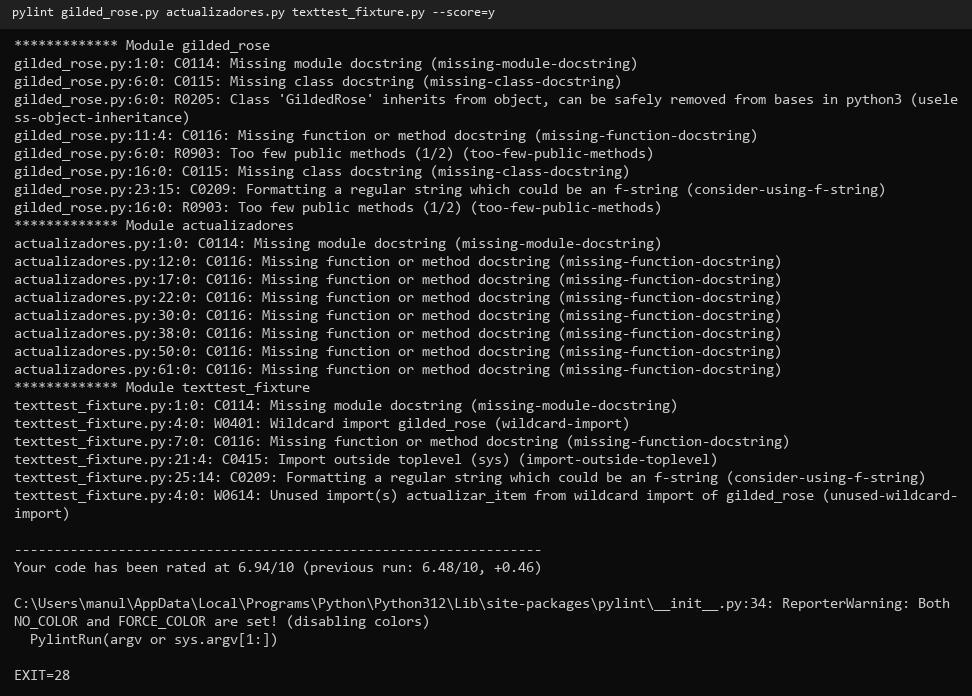
\includegraphics[width=\textwidth]{imagenes/06_pylint_despues.png}
\caption{Salida de pylint después de la refactorización.}
\label{fig:pylint-despues}
\end{figure}

\begin{figure}[!htbp]
\centering
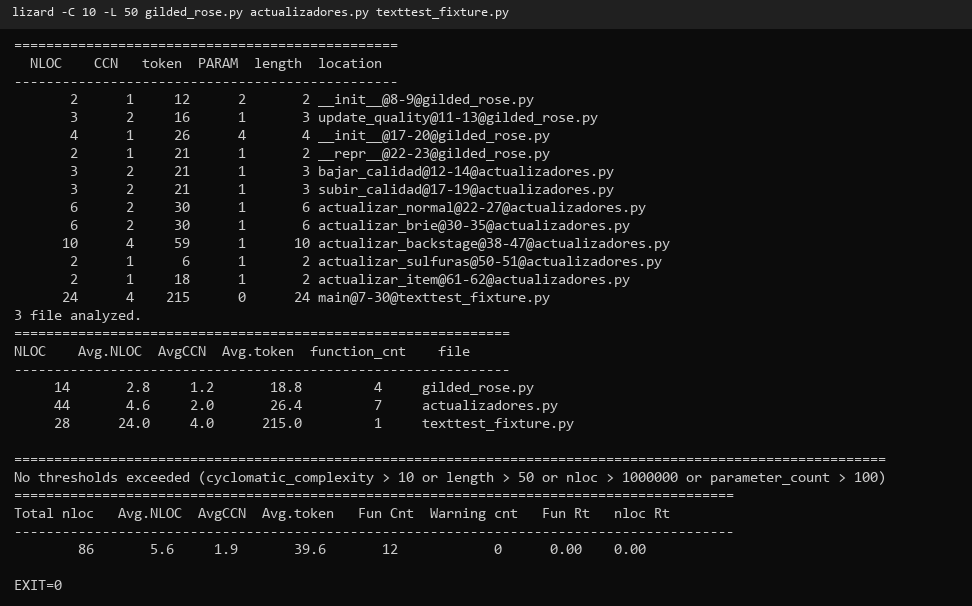
\includegraphics[width=\textwidth]{imagenes/07_lizard_despues.png}
\caption{Salida de lizard después de la refactorización.}
\label{fig:lizard-despues}
\end{figure}

\section{Control de versiones}
Repositorio público: \url{https://github.com/Manulol1904/gilded-rose-mantenimiento}. Rama \texttt{main}. La refactorización vivió en \texttt{refactor/gilded-rose}. La integración fue un merge \texttt{--no-ff}, commit \texttt{5dbd777}, mensaje \texttt{merge: integrar refactorización de GildedRose}, con dos padres. El tag \texttt{v1.0-refactor} apunta a ese merge. Figuras~\ref{fig:ramas} y~\ref{fig:grafo}. La página del repositorio y el listado de ramas están en las figuras~\ref{fig:github-repo} y~\ref{fig:github-ramas}.

\begin{figure}[!htbp]
\centering
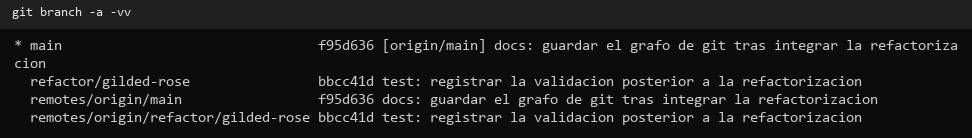
\includegraphics[width=\textwidth]{imagenes/11_git_branches.png}
\caption{Salida de \texttt{git branch -a -vv}.}
\label{fig:ramas}
\end{figure}

\begin{figure}[!htbp]
\centering
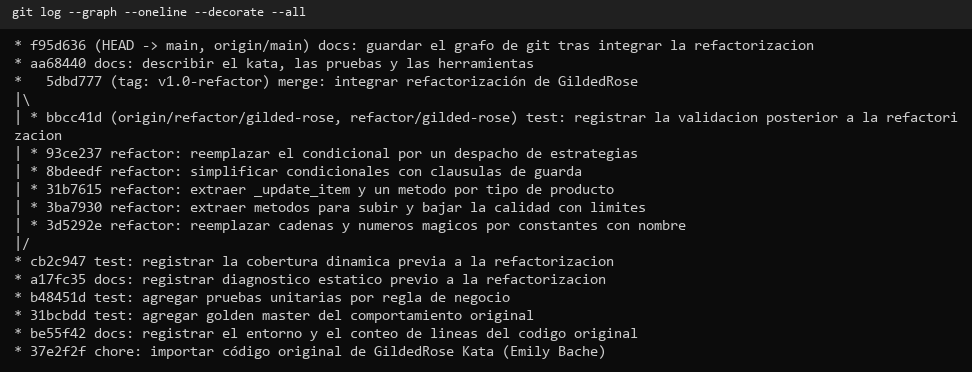
\includegraphics[width=\textwidth]{imagenes/12_git_log_graph_merge.png}
\caption{Salida de \texttt{git log --graph --oneline --decorate --all}.}
\label{fig:grafo}
\end{figure}

\begin{figure}[!htbp]
\centering
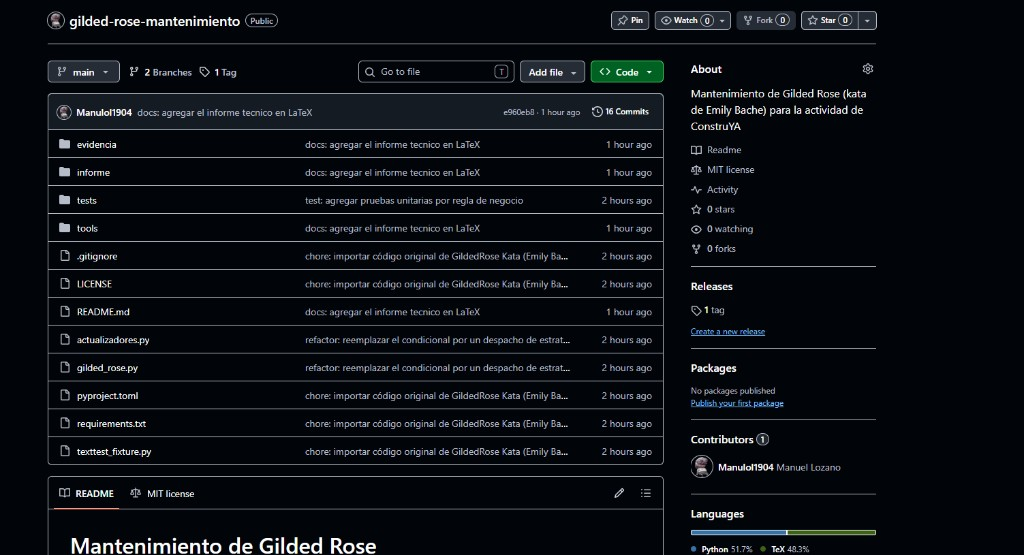
\includegraphics[width=\textwidth,height=0.38\textheight,keepaspectratio]{imagenes/13_github_repo.png}
\caption{Captura manual de la página del repositorio público en GitHub.}
\label{fig:github-repo}
\end{figure}

\begin{figure}[!htbp]
\centering
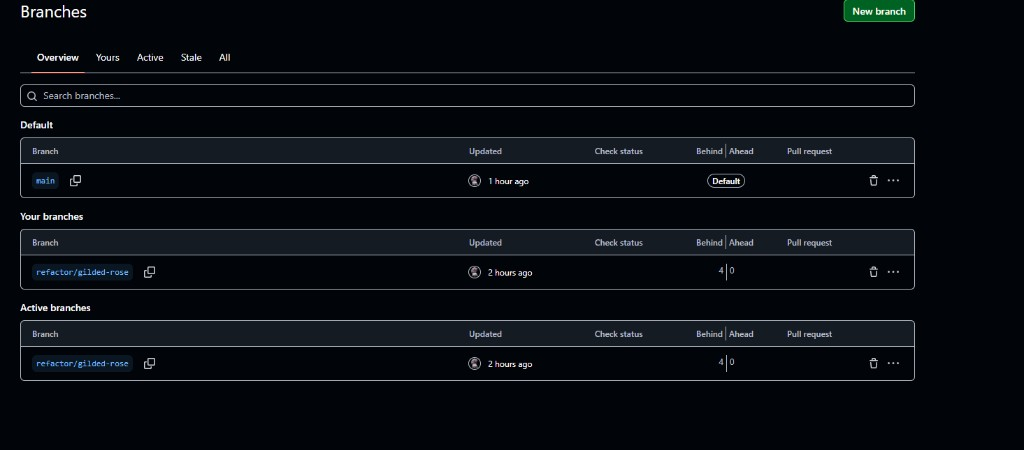
\includegraphics[width=\textwidth,height=0.32\textheight,keepaspectratio]{imagenes/14_github_ramas.png}
\caption{Captura manual de las ramas \texttt{main} y \texttt{refactor/gilded-rose} en GitHub.}
\label{fig:github-ramas}
\end{figure}

\section{Pruebas y validación}
unittest, 11 pruebas de regla y 2 de golden master. El ítem normal baja 1; vencido, baja 2; la calidad no pasa de 0 ni de 50; Aged Brie sube; Sulfuras no cambia; Backstage sube 1, 2 o 3 según le falten más de 10, 10 o menos, o 5 o menos días, y cae a 0 tras el concierto. ``Conjured Mana Cake'' baja 1, igual que un ítem normal. El golden master compara 5833 combinaciones y 40 días contra \texttt{tests/golden\_master.json}. \texttt{git diff} de ese archivo no tiene líneas (figura~\ref{fig:diff}). Antes y después, las 13 pruebas pasan (figuras~\ref{fig:test-antes} y~\ref{fig:test-despues}).

\begin{figure}[!htbp]
\centering
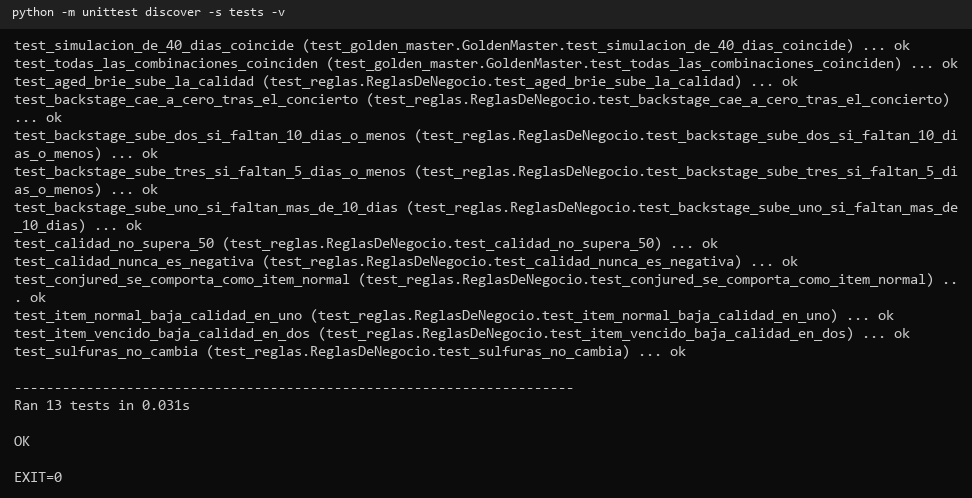
\includegraphics[width=\textwidth]{imagenes/04_unittest_antes.png}
\caption{Salida de \texttt{python -m unittest discover -s tests -v} antes de refactorizar.}
\label{fig:test-antes}
\end{figure}

\begin{figure}[!htbp]
\centering
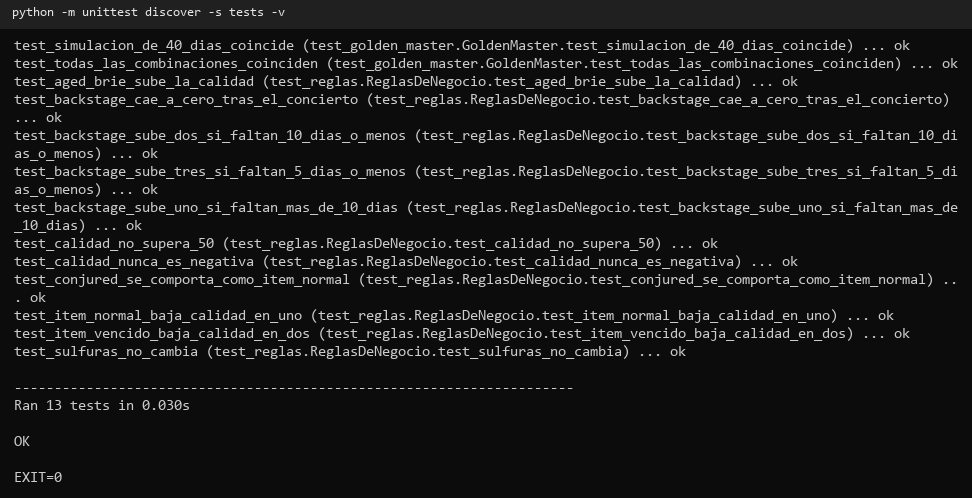
\includegraphics[width=\textwidth]{imagenes/08_unittest_despues.png}
\caption{Salida del mismo comando de unittest después de refactorizar.}
\label{fig:test-despues}
\end{figure}

\begin{figure}[!htbp]
\centering
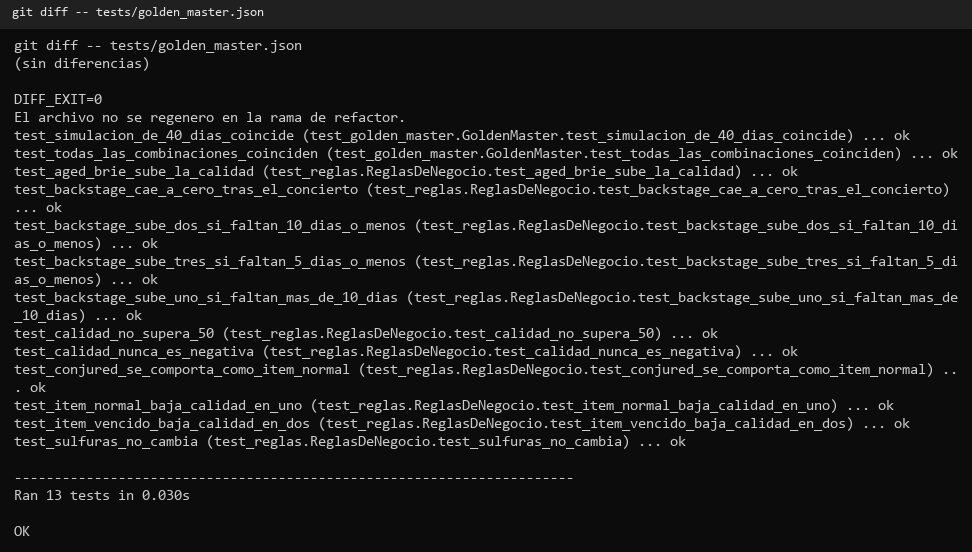
\includegraphics[width=\textwidth]{imagenes/10_golden_master_diff.png}
\caption{Salida de \texttt{git diff -- tests/golden\_master.json}: el archivo no cambió.}
\label{fig:diff}
\end{figure}

\section{Limitaciones y trabajo futuro}
No se implementó la regla Conjured: hoy ese nombre sigue el camino del ítem normal, y cambiarlo modificaría el comportamiento fijado por las pruebas. \texttt{Item} sigue siendo la clase original. \texttt{texttest\_fixture.py} conserva el import estrella. Las funciones nuevas no tienen docstring, y por eso pylint cuenta más avisos aunque la nota sube.

\section{Reflexión sobre calidad y sostenibilidad}
El cambio baja el costo de una regla nueva. Aged Brie, Sulfuras y Backstage ya no comparten un condicional de seis niveles: cada uno tiene una función, y el golden master avisa si la salida se mueve. Eso reduce el riesgo de una falla al mantener el inventario. El límite es el que las pruebas fijan el comportamiento actual, incluido el de Conjured. Una solicitud equivalente a la pasarela de pagos de ConstruYA, por ejemplo otra familia de productos, debería entrar como otra estrategia y con pruebas propias, no como otra rama dentro de \texttt{update\_quality}. La deuda que queda está localizada: la clase \texttt{Item} no se toca y la regla Conjured sigue pendiente.

\section{Contraste con la rúbrica}
\begin{center}
\scriptsize
\begin{tabular}{|p{2.3cm}|p{12.6cm}|}
\hline
Criterio & Dónde se evidencia \\
\hline
C1 Diagnóstico & Sección 2, figuras~\ref{fig:pylint-antes} y~\ref{fig:lizard-antes}, \texttt{evidencia/diagnostico\_smells.txt}. Seis smells. \\
\hline
C2 Refactorización & Sección 3. Cinco técnicas, antes y después. El golden master no cambió. \\
\hline
C3 Herramientas & Sección 4. Estática: pylint y lizard. Dinámica: coverage.py con ramas. \\
\hline
C4 Git & Sección 5, figuras~\ref{fig:ramas}, \ref{fig:grafo}, \ref{fig:github-repo} y~\ref{fig:github-ramas}. Rama, commits atómicos, merge \texttt{5dbd777} y tag \texttt{v1.0-refactor}. \\
\hline
C5 Pruebas & Sección 6, figuras~\ref{fig:test-antes}, \ref{fig:test-despues} y~\ref{fig:diff}. Trece pruebas y diff vacío. \\
\hline
\end{tabular}
\end{center}

\end{document}
